%% Ankur Sinha

%% packages %%
% support for coloured text
\usepackage{color}
% IPA
\usepackage{tipa}
\usepackage[scale=2]{ccicons}
\usepackage{amssymb}
\usepackage{tikz}
\usetikzlibrary{arrows.meta, arrows}
\usepackage{pgfplots}
\pgfmathdeclarefunction{gaussnew}{4}{%nu, eta, eps, omega
  \pgfmathparse{(#1*((2*exp(-(((x-((#2+#3)/2))/((#2-#3)/(2*sqrt(-ln(#4/2)))))^2))) -#4))}%chktex 36
}
\usepackage{jneurosci}
\usepackage{subfig}
\usepackage[T1]{fontenc}
\usepackage[utf8]{inputenc}
\usepackage[style=nature,backend=biber,autocite=footnote]{biblatex}
\addbibresource{/home/asinha/Documents/01_Readables/00_research_papers/masterbib.bib}
% Use opensans
\usepackage[default,osfigures,scale=0.95]{opensans}
% for strike through
\usepackage[normalem]{ulem}
% links, urls, refs
\definecolor{links}{HTML}{2A1B81}
% Fedora blue for the theme
\definecolor{FedoraBlue}{HTML}{2A1B81}
\usepackage{hyperref}
\hypersetup{colorlinks,linkcolor=Green,urlcolor=links}
% graphics
\usepackage{graphicx}
% algorithm
\usepackage{algorithmic}
\usepackage{textcomp}
\usepackage{wrapfig}
\usepackage{textgreek}
\usepackage{euler}

% beamer theme
% use defaults for theme
\usetheme[numbering=fraction]{metropolis}
\usefonttheme[onlymath]{serif}
\setbeamerfont{footnote}{size=\tiny}
\setbeamerfont{caption}{size=\tiny}
\setbeamercolor{alerted text}{fg=Green}
\setbeamerfont{note page}{size=\small}

% Not needed in metropolis, but in general footnote citation fixes: https://tex.stackexchange.com/questions/44217/how-can-i-stop-footcite-from-hijacking-my-beamer-columns
% how to use multiple references to the same footnote: https://tex.stackexchange.com/questions/27763/beamer-multiple-references-to-the-same-footnote

%% title %%
\title{\centering Investigating activity dependent dynamics of synaptic structures using biologically plausible models of post-deafferentation network repair\\}
\subtitle{\centering
\includegraphics[width=0.2\textwidth]{99_images/UH-IT-theme.png}\\
\includegraphics[scale=0.6]{99_images/UH-Logo-Black.eps}\\\vspace{0.2cm}Engineering and Computer Science Conference, 2019\\}
\author[Ankur Sinha]{Ankur Sinha, UH Biocomputation Group}
\date{17/04/2019}

%% document begins %%
\begin{document}

% title frame %%
\begin{frame}
  \titlepage{}
\end{frame}

%% Three slides for 5 minutes seems good
%% So, 6 slides for 10 minutes
\section{The brain: learning, plasticity, stability}
\begin{frame}[c]{The brain: in numbers}
  
\end{frame}
\begin{frame}[c]{The brain: learning and plasticity}
  
\end{frame}

\begin{frame}[c]{The brain: plasticity while homeostasis}
\end{frame}

\section{Studying homeostatic processes}
\begin{frame}[c]{Experimental protocol I}
  \note[item]{The protocol is pretty standard. Here, for a study in the visual cortex, the retinal field of a rat or a mouse is mapped.}
  \begin{columns}
    \begin{column}{0.5\textwidth}
      \centering
      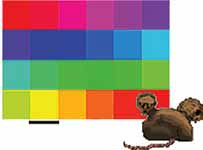
\includegraphics[width=0.8\textwidth]{99_images/keck-1-1a}%chktex 8
    \end{column}
    \begin{column}{0.5\textwidth}
      \centering
      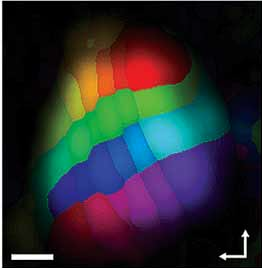
\includegraphics[width=0.8\textwidth]{99_images/keck-1-1c}%chktex 8
    \end{column}
  \end{columns}
  \footnotetext[1]{\fullcite{Keck2008}}
\end{frame}

\begin{frame}[c]{Experimental protocol II:\ after peripheral lesion}
  \note[item]{Then, a part of the retina is lesioned. This cuts off inputs to a part of the visual cortex, as shown in the first figure. This forms the Lesion Projection Zone (LPZ). By repeated imaging of the region over months, the reorganisation of the network is tracked.}
  \note[item]{Other lesion studies use similar methods: digit removal, whisker trimming, and so on---anything that cuts off projecting activity on to a set of neurons.}
    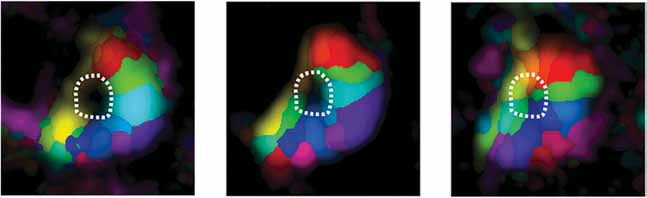
\includegraphics[width=\textwidth]{99_images/keck-1-2c}%chktex 8
    \footnotetext[1]{\fullcite{Keck2008}}
\end{frame}
\section{Our model}
\begin{frame}[c]{Simulation protocol}
  \begin{figure}[h]
    \centering
    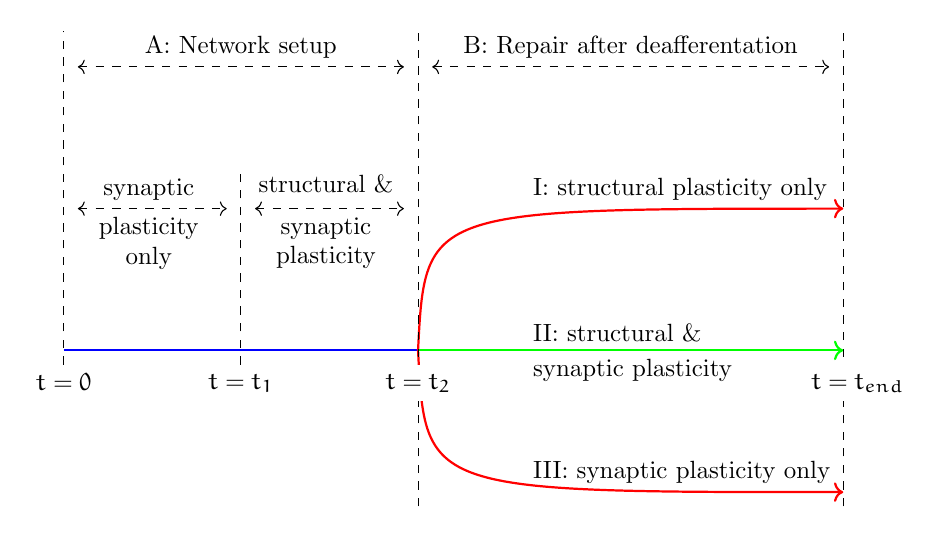
\begin{tikzpicture}[scale=0.9, transform shape]

  % horizontal lines
  \draw[blue, thick] (0,4) -- (5,4);
  \draw[green, thick, ->] (5,4) -- (11,4);
  \draw[red, thick, ->] (5,4) .. controls (5.1,6) .. (11,6);
  \draw[red, thick, ->] (5,4) .. controls (5.1,2) .. (11,2);


  \draw[dashed] (0,3.8) -- (0,8.5);
  \node[below] at (0, 3.8)  {\(t=0\)};

  \draw[dashed] (2.5,3.8) -- (2.5,6.5);
  \node[below] at (2.5, 3.8)  {\(t=t_1\)};

  \draw[dashed, -] (5,1.8) -- (5,8.5);
  \node[below, fill=white] at (5, 3.8)  {\(t=t_2\)};

  \draw[dashed] (11,1.8) -- (11,8.5);
  \node[below, fill=white] at (11.2, 3.8)  {\(t=t_{end}\)};

  \draw[dashed, <->] (0.2,8) -- (4.8,8);
  \node[above] at (2.5,8) {A: Network setup};

  \draw[dashed, <->] (0.2,6) -- (2.3,6);
  \node[above] at (1.2,6) {synaptic};
  \node[below, align=center] at (1.2,6) {plasticity\\only};
  \draw[dashed, <->] (2.7,6) -- (4.8,6);
  \node[above] at (3.7,6.1) {structural \&};
  \node[below, align=center] at (3.7,6) {synaptic\\plasticity};

  \draw[dashed, <->] (5.2,8) -- (10.8,8);
  \node[above] at (8,8) {B: Repair after deafferentation};


  \node[above right, align=left] at (6.5,6) {I: structural plasticity only};
  \node[above right, align=left] at (6.5,4) {II: structural \&};
  \node[below right, align=left] at (6.5,4) {synaptic plasticity};
  \node[above right, align=left] at (6.5,2) {III: synaptic plasticity only};

\end{tikzpicture}

  \end{figure}
  \note[item]{Explain the simulation protocol.}
\end{frame}
\section{Results and discussion}
\begin{frame}[c]{Deafferentation and successful repair}
  \begin{figure}
      \centering
      \resizebox{\textwidth}{!}{% GNUPLOT: LaTeX picture with Postscript
\begingroup
  \makeatletter
  \providecommand\color[2][]{%
    \GenericError{(gnuplot) \space\space\space\@spaces}{%
      Package color not loaded in conjunction with
      terminal option `colourtext'%
    }{See the gnuplot documentation for explanation.%
    }{Either use 'blacktext' in gnuplot or load the package
      color.sty in LaTeX.}%
    \renewcommand\color[2][]{}%
  }%
  \providecommand\includegraphics[2][]{%
    \GenericError{(gnuplot) \space\space\space\@spaces}{%
      Package graphicx or graphics not loaded%
    }{See the gnuplot documentation for explanation.%
    }{The gnuplot epslatex terminal needs graphicx.sty or graphics.sty.}%
    \renewcommand\includegraphics[2][]{}%
  }%
  \providecommand\rotatebox[2]{#2}%
  \@ifundefined{ifGPcolor}{%
    \newif\ifGPcolor
    \GPcolortrue
  }{}%
  \@ifundefined{ifGPblacktext}{%
    \newif\ifGPblacktext
    \GPblacktexttrue
  }{}%
  % define a \g@addto@macro without @ in the name:
  \let\gplgaddtomacro\g@addto@macro
  % define empty templates for all commands taking text:
  \gdef\gplbacktext{}%
  \gdef\gplfronttext{}%
  \makeatother
  \ifGPblacktext
    % no textcolor at all
    \def\colorrgb#1{}%
    \def\colorgray#1{}%
  \else
    % gray or color?
    \ifGPcolor
      \def\colorrgb#1{\color[rgb]{#1}}%
      \def\colorgray#1{\color[gray]{#1}}%
      \expandafter\def\csname LTw\endcsname{\color{white}}%
      \expandafter\def\csname LTb\endcsname{\color{black}}%
      \expandafter\def\csname LTa\endcsname{\color{black}}%
      \expandafter\def\csname LT0\endcsname{\color[rgb]{1,0,0}}%
      \expandafter\def\csname LT1\endcsname{\color[rgb]{0,1,0}}%
      \expandafter\def\csname LT2\endcsname{\color[rgb]{0,0,1}}%
      \expandafter\def\csname LT3\endcsname{\color[rgb]{1,0,1}}%
      \expandafter\def\csname LT4\endcsname{\color[rgb]{0,1,1}}%
      \expandafter\def\csname LT5\endcsname{\color[rgb]{1,1,0}}%
      \expandafter\def\csname LT6\endcsname{\color[rgb]{0,0,0}}%
      \expandafter\def\csname LT7\endcsname{\color[rgb]{1,0.3,0}}%
      \expandafter\def\csname LT8\endcsname{\color[rgb]{0.5,0.5,0.5}}%
    \else
      % gray
      \def\colorrgb#1{\color{black}}%
      \def\colorgray#1{\color[gray]{#1}}%
      \expandafter\def\csname LTw\endcsname{\color{white}}%
      \expandafter\def\csname LTb\endcsname{\color{black}}%
      \expandafter\def\csname LTa\endcsname{\color{black}}%
      \expandafter\def\csname LT0\endcsname{\color{black}}%
      \expandafter\def\csname LT1\endcsname{\color{black}}%
      \expandafter\def\csname LT2\endcsname{\color{black}}%
      \expandafter\def\csname LT3\endcsname{\color{black}}%
      \expandafter\def\csname LT4\endcsname{\color{black}}%
      \expandafter\def\csname LT5\endcsname{\color{black}}%
      \expandafter\def\csname LT6\endcsname{\color{black}}%
      \expandafter\def\csname LT7\endcsname{\color{black}}%
      \expandafter\def\csname LT8\endcsname{\color{black}}%
    \fi
  \fi
    \setlength{\unitlength}{0.0500bp}%
    \ifx\gptboxheight\undefined%
      \newlength{\gptboxheight}%
      \newlength{\gptboxwidth}%
      \newsavebox{\gptboxtext}%
    \fi%
    \setlength{\fboxrule}{0.5pt}%
    \setlength{\fboxsep}{1pt}%
\begin{picture}(7936.00,2550.00)%
    \gplgaddtomacro\gplbacktext{%
    }%
    \gplgaddtomacro\gplfronttext{%
    }%
    \gplgaddtomacro\gplbacktext{%
    }%
    \gplgaddtomacro\gplfronttext{%
    }%
    \gplgaddtomacro\gplbacktext{%
    }%
    \gplgaddtomacro\gplfronttext{%
    }%
    \gplgaddtomacro\gplbacktext{%
    }%
    \gplgaddtomacro\gplfronttext{%
      \csname LTb\endcsname%
      \put(7554,51){\makebox(0,0)[l]{\strut{}$1$}}%
      \put(7554,2285){\makebox(0,0)[l]{\strut{}$5$}}%
      \put(7752,1168){\rotatebox{-270}{\makebox(0,0){\strut{}Firing rate (Hz)}}}%
    }%
    \gplbacktext
    \put(0,0){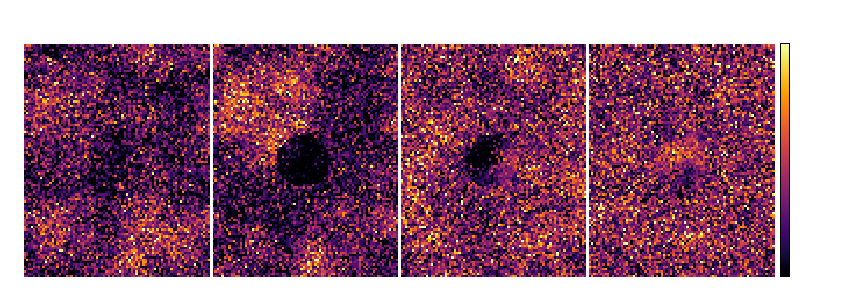
\includegraphics[interpolate=false]{99_images/201811221433-firing-rate-snapshots-E}}%
    \gplfronttext
  \end{picture}%
\endgroup
}%
  \end{figure}
\end{frame}
\begin{frame}[c]{Conclusions}
  \begin{itemize}
    \item New model: biologically realistic.
      \pause{}
    \item Replicates experimental observations:
      \pause{}
    \item Suggests:
      \begin{itemize}
        \item Activity dependent dynamics for synaptic structures.
        \item Single neuron stabilisation by structural plasticity.
      \end{itemize}
  \end{itemize}
\end{frame}
\begin{frame}[c]{Now what?}
  \begin{itemize}
    \item Functional implications of structural plasticity? Associative memory?
      \pause{}
    \item Application of growth dynamics to multi-compartmental neuron models?
      \pause{}
    \item Faithful modelling of cytoskeleton modification (actin)?
  \end{itemize}
\end{frame}
\end{document}
